\documentclass[17pt]{article}

\usepackage[margin=1in, paperwidth=8.5in, paperheight=11in]{geometry}
\usepackage{amsmath}
\usepackage[document]{ragged2e}
\usepackage{graphicx}
\usepackage{listings}
\usepackage{color}
\usepackage[none]{hyphenat}

\definecolor{dkgreen}{rgb}{0,0.6,0}
\definecolor{gray}{rgb}{0.5,0.5,0.5}
\definecolor{mauve}{rgb}{0.58,0,0.82}

\lstset{frame=tb,
  language=Python,
  aboveskip=3mm,
  belowskip=3mm,
  showstringspaces=false,
  columns=flexible,
  basicstyle={\small\ttfamily},
  numbers=none,
  numberstyle=\tiny\color{gray},
  keywordstyle=\color{blue},
  commentstyle=\color{dkgreen},
  stringstyle=\color{mauve},
  breaklines=true,
  breakatwhitespace=true,
  tabsize=3
}

\begin{document}

\title{{Bayesean Data Analysis - Exercise 7}}
\maketitle


\section{Linear model: drowning data with Stan}
This is how the modified Stan code looks like: \\
\begin{lstlisting}
data {
    int <lower=0> N; //number of data points
    vector[N] x; //observation year
    vector[N] y; //observation number of drowned
    real xpred; //prediction year
    real pmubeta;
    real psbeta;
}

parameters {
    real alpha;
    real beta;
    real <lower=0> sigma;
}

transformed parameters {
    vector[N] mu;
    mu = alpha + beta*x;
}

model {
    beta ~ normal(pmubeta, psbeta);
    y ~ normal(mu, sigma);
}

generated quantities {
    real ypred;
    ypred = normal_rng(alpha + beta*xpred, sigma);
}
\end{lstlisting}

The code that was provided for us has two mistakes in it. \\
The first one is in the declaration of \textbf{sigma}: \\
\begin{lstlisting}
real sigma;
\end{lstlisting}
which is not correct because the standard deviation can't have negative values and needs to have a lower bound of 0. \\
Here is how we fix that: \\
\begin{lstlisting}
real <lower=0> sigma;
\end{lstlisting}
The second mistake is in the calculation of the \textbf{ypred}, where it is given as: \\
\begin{lstlisting}
ypred = normal_rng(mu, sigma);
\end{lstlisting}
and it should be modified to look like this: \\
\begin{lstlisting}
ypred = normal_rng(alpha + beta*xpred, sigma);
\end{lstlisting}
because it is a linear model and the formula should be $ y = a + bx$.
\\~\\~\\
It is also stated that we should use weakly informative prior $N(0, \tau^2)$.
The $\tau$ value that I am using is \textbf{26.788}.

The $\tau$ value is calculated with the following Python code: \\
\begin{lstlisting}
alpha_val = 0
tau = 26.788
beta_val = tau
prior = norm(alpha_val, beta_val)
a = np.arange(-1000, 1000, 0.1)
b = prior.pdf(a)
print(prior.interval(0.99))
\end{lstlisting}
The prior is implemented in the following way: \\
First we declare mean and std for beta in the \textbf{data} block as follows: \\
\begin{lstlisting}
real pmubeta;
real psbeta;
\end{lstlisting}
then in the \textbf{model} block we calculate beta: \\
\begin{lstlisting}
beta ~ normal(pmubeta, psbeta);
\end{lstlisting}
We also need to add it as a parameter in the \textbf{parameter} block:
\begin{lstlisting}
real beta;
\end{lstlisting}
From the prediction we can see that the predicted value from drownings in 2019 is \textbf{120}. \\
We can also that the number of drownings is \textbf{decreasing} every year.

\newpage

\begin{align}
\textbf{SOURCE CODE}
\end{align}

\begin{lstlisting}
import pystan
import numpy as np
import pandas as pd
from scipy.stats import norm, beta
import matplotlib.pyplot as plt
import matplotlib as mpl

df = pd.read_csv('drowning.csv', sep=' ', header=None)
year = df[0].values
number_deaths = df[1].values
number_datapoints = len(df)
prediction_year = 2019

alpha_val = 0
tau = 26.788
beta_val = tau
prior = norm(alpha_val, beta_val)
a = np.arange(-1000, 1000, 0.1)
b = prior.pdf(a)
print(prior.interval(0.99))


drowning_code = '''
data {
    int <lower=0> N; //number of data points
    vector[N] x; //observation year
    vector[N] y; //observation number of drowned
    real xpred; //prediction year
    real pmubeta;
    real psbeta;
}

parameters {
    real alpha;
    real beta;
    real <lower=0> sigma;
}

transformed parameters {
    vector[N] mu;
    mu = alpha + beta*x;
}

model {
    beta ~ normal(pmubeta, psbeta);
    y ~ normal(mu, sigma);
}

generated quantities {
    real ypred;
    ypred = normal_rng(alpha + beta*xpred, sigma);
}
'''

drowning_data = {'N': number_datapoints,
                'x': year,
                'y': number_deaths,
                 'xpred': prediction_year,
                 'pmubeta': 0,
                 'psbeta': tau
                 
               }

sm = pystan.StanModel(model_code = drowning_code)
fit = sm.sampling(data = drowning_data)
\end{lstlisting}

\newpage
\section{Hierarchical model: factory data with Stan}
\subsection{Separate model}
Here is that Stan code for the separate model:
\begin{lstlisting}
data {
    int<lower=0> N; // number of data points
    int<lower=0> K; // number of groups
    int<lower=1,upper=K> x[N]; // group indicator
    vector[N] y; //
}

parameters {
    vector[K] mu;         // group means
    //real<lower=0> sigma;
    vector<lower=0>[K] sigma;
}

model {
  y ~ normal(mu[x], sigma[x]);
}

generated quantities {
    real ypred;
    ypred = normal_rng(mu[6], sigma[6]);
}
\end{lstlisting}

The posterior mean for the sixth machine is \textbf{86.341}\\
\begin{center}
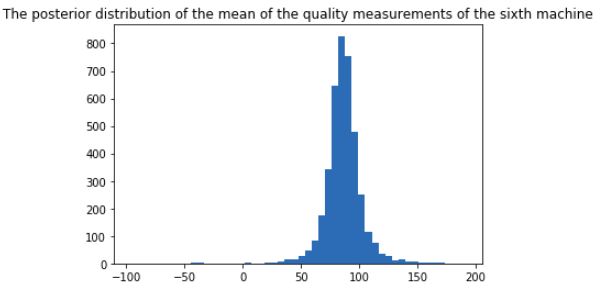
\includegraphics[width=15cm, height=7cm]{mean_separate.png}
\end{center}

\newpage

The mean for another quality measurement of the sixth machine is \textbf{86.322}
\begin{center}
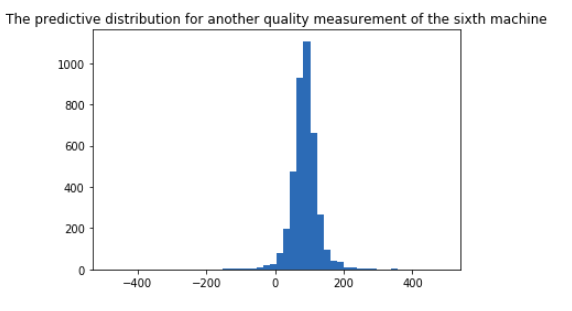
\includegraphics[width=15cm, height=7cm]{next_separate.png}
\end{center}

The posterior distribution of the mean of the quality measurements of the seventh machine can't be calculated because we are calculating for every machine separately and there is not data for the seventh machine.

\subsection{Pooled model}
Here is that Stan code for the pooled model:
\begin{lstlisting}
data {
    int<lower=0> N; // number of data points
    vector[N] y;
}

parameters {
    real mu;             // prior mean
    real<lower=0> sigma;
}

model {
  y ~ normal(mu, sigma);
}

generated quantities {
    real ypred;
    ypred = normal_rng(mu, sigma);
}
\end{lstlisting}

\newpage
The posterior mean for the sixth machine is \textbf{92.903}\\
\begin{center}
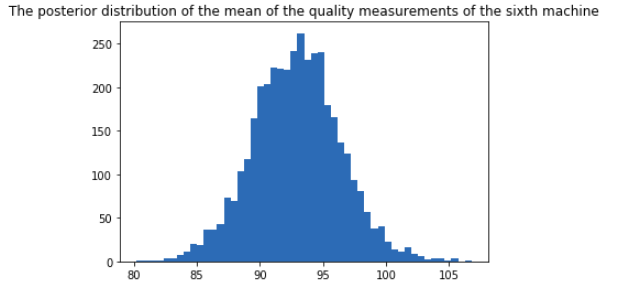
\includegraphics[width=15cm, height=7cm]{mean_pooled.png}
\end{center}

The mean for another quality measurement of the sixth machine is \textbf{92.637}
\begin{center}
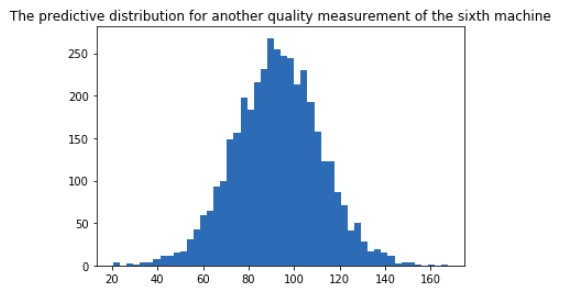
\includegraphics[width=15cm, height=7cm]{next_pooled.png}
\end{center}

The posterior distribution of the mean of the quality measurements of the seventh machine is the same and for the sixth machine because all the measurements are combined together.

\subsection{Hierarchical model}
Here is that Stan code for the hierarchical model:
\begin{lstlisting}
data {
    int<lower=0> N; // number of data points
    int<lower=0> K; // number of groups
    int<lower=1,upper=K> x[N]; // group indicator
    vector[N] y; //
}

parameters {
    real mu0;             // prior mean
    real<lower=0> sigma0; // prior std
    
    vector[K] mu;         // group means
    real<lower=0> sigma;
}

model {
    mu ~ normal(mu0, sigma0);
    y ~ normal(mu[x], sigma);
}

generated quantities {
    real mu7;
    real ypred6;
    
    mu7 = normal_rng(mu0, sigma0);
    ypred6 = normal_rng(mu[6], sigma);
}
\end{lstlisting}

The posterior mean for the sixth machine is \textbf{87.456}\\
\begin{center}
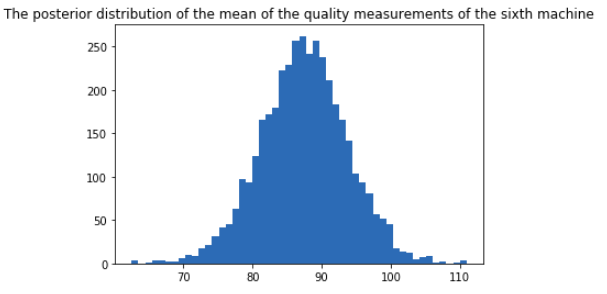
\includegraphics[width=15cm, height=7cm]{mean_hierarchical.png}
\end{center}

The mean for another quality measurement of the sixth machine is \textbf{87.528}
\begin{center}
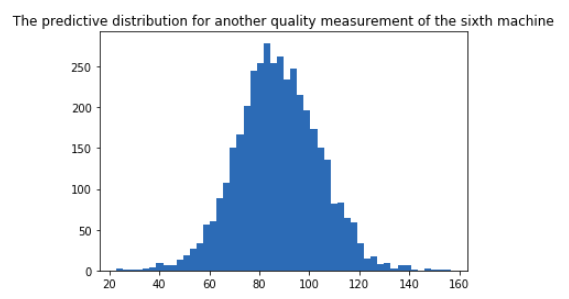
\includegraphics[width=15cm, height=7cm]{next_hierarchical.png}
\end{center}

\newpage

The posterior distribution of the mean of the quality measurements of the seventh machine is \textbf{93.037}.

\begin{center}
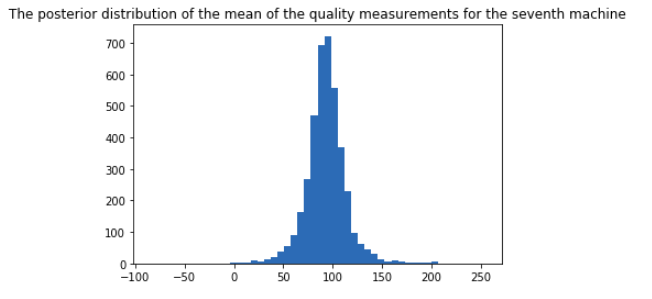
\includegraphics[width=15cm, height=7cm]{seventh_machine.png}
\end{center}


\newpage

\begin{align}
\textbf{SOURCE CODE}
\end{align}

\begin{lstlisting}
import pystan
import numpy as np
import pandas as pd
from scipy.stats import norm, beta
import matplotlib.pyplot as plt
import matplotlib as mpl


# POOLED MODEL
df = pd.read_csv('factory.csv', sep=' ', header=None)
number_datapoints = df.shape[0] * df.shape[1]
# num_groups = df.shape[1]
y = df.values
y = y.ravel()
x = np.arange(1, df.shape[1]+1, 1)

pooled_factory_code = '''
data {
    int<lower=0> N; // number of data points
    vector[N] y;
}

parameters {
    real mu;             // prior mean
    real<lower=0> sigma;
}

model {
  y ~ normal(mu, sigma);
}

generated quantities {
    real ypred;
    ypred = normal_rng(mu, sigma);
}
'''


pooled_factory_data = {'N': number_datapoints,
                'y': y
               }

sm = pystan.StanModel(model_code = pooled_factory_code)
pooled_fit = sm.sampling(data = pooled_factory_data)


summary = pooled_fit.summary()
summary = pd.DataFrame(summary['summary'], columns=summary['summary_colnames'], index=summary['summary_rownames'])

mu6 = pooled_fit.extract(permuted=True)['mu']
plt.hist(mu6, bins=50)
plt.title('The posterior distribution of the mean of the quality measurements of the sixth machine')
plt.show()

ypred = pooled_fit.extract(permuted=True)['ypred']
plt.hist(ypred, bins=50)
plt.title('The predictive distribution for another quality measurement of the sixth machine')
plt.show()
summary


# HIERARCHICAL MODEL
df = pd.read_csv('factory.csv', sep=' ', header=None)
number_datapoints = df.shape[0] * df.shape[1]
num_groups = df.shape[1]
y = df.values
y = np.reshape(y, 30, order='F')
y = y.ravel()
x = np.arange(1,7)
x = np.repeat(x, 5)

hierarchical_factory_code = '''
data {
    int<lower=0> N; // number of data points
    int<lower=0> K; // number of groups
    int<lower=1,upper=K> x[N]; // group indicator
    vector[N] y; //
}

parameters {
    real mu0;             // prior mean
    real<lower=0> sigma0; // prior std
    
    vector[K] mu;         // group means
    real<lower=0> sigma;
}

model {
    mu ~ normal(mu0, sigma0);
    y ~ normal(mu[x], sigma);
}

generated quantities {
    real mu7;
    real ypred6;
    
    mu7 = normal_rng(mu0, sigma0);
    ypred6 = normal_rng(mu[6], sigma);
}
'''

hierarchical_factory_data = {'N': number_datapoints,
                'K': num_groups,
                'x': x,
                'y': y
               }

sm = pystan.StanModel(model_code = hierarchical_factory_code)
hierarchical_fit = sm.sampling(data = hierarchical_factory_data)


summary = hierarchical_fit.summary()
summary = pd.DataFrame(summary['summary'], columns=summary['summary_colnames'], index=summary['summary_rownames'])

mu6 = hierarchical_fit.extract(permuted=True)['mu'][:,5]
plt.hist(mu6, bins=50)
plt.title('The posterior distribution of the mean of the quality measurements of the sixth machine')
plt.show()


ypred6 = hierarchical_fit.extract(permuted=True)['ypred6']
plt.hist(ypred6, bins=50)
plt.title('The predictive distribution for another quality measurement of the sixth machine')
plt.show()


mu7 = hierarchical_fit.extract(permuted=True)['mu7']
plt.hist(mu7, bins=50)
plt.title('The posterior distribution of the mean of the quality measurements for the seventh machine')
plt.show()

summary


# SEPARATE MODEL
df = pd.read_csv('factory.csv', sep=' ', header=None)
number_datapoints = df.shape[0] * df.shape[1]
num_groups = df.shape[1]
y = df.values
y = np.reshape(y, 30, order='F')
y = y.ravel()
x = np.arange(1,7)
x = np.repeat(x, 5)


separate_factory_code = '''
data {
    int<lower=0> N; // number of data points
    int<lower=0> K; // number of groups
    int<lower=1,upper=K> x[N]; // group indicator
    vector[N] y; //
}

parameters {
    vector[K] mu;         // group means
    //real<lower=0> sigma;
    vector<lower=0>[K] sigma;
}

model {
  y ~ normal(mu[x], sigma[x]);
}

generated quantities {
    real ypred;
    ypred = normal_rng(mu[6], sigma[6]);
}
'''

separate_factory_data = {'N': number_datapoints,
                'K': num_groups,
                'x': x,
                'y': y
               }

sm = pystan.StanModel(model_code = separate_factory_code)
separate_fit = sm.sampling(data = separate_factory_data)


summary = separate_fit.summary()
summary = pd.DataFrame(summary['summary'], columns=summary['summary_colnames'], index=summary['summary_rownames'])

mu6 = separate_fit.extract(permuted=True)['mu'][:, 5]
plt.hist(mu6, bins=50)
plt.title('The posterior distribution of the mean of the quality measurements of the sixth machine')
plt.show()

ypred = separate_fit.extract(permuted=True)['ypred']
plt.hist(ypred, bins=50)
plt.title('The predictive distribution for another quality measurement of the sixth machine')
plt.show()
summary
\end{lstlisting}


\end{document}








